
\subsection{Pre-processing}

\subsection{Segmentation using Supervised Graph Embedding}

\subsection{Obtaining Glomerular Count}


%\begin{figure*}[t]
%\begin{minipage}[b]{0.99\linewidth}
%  \centering
%  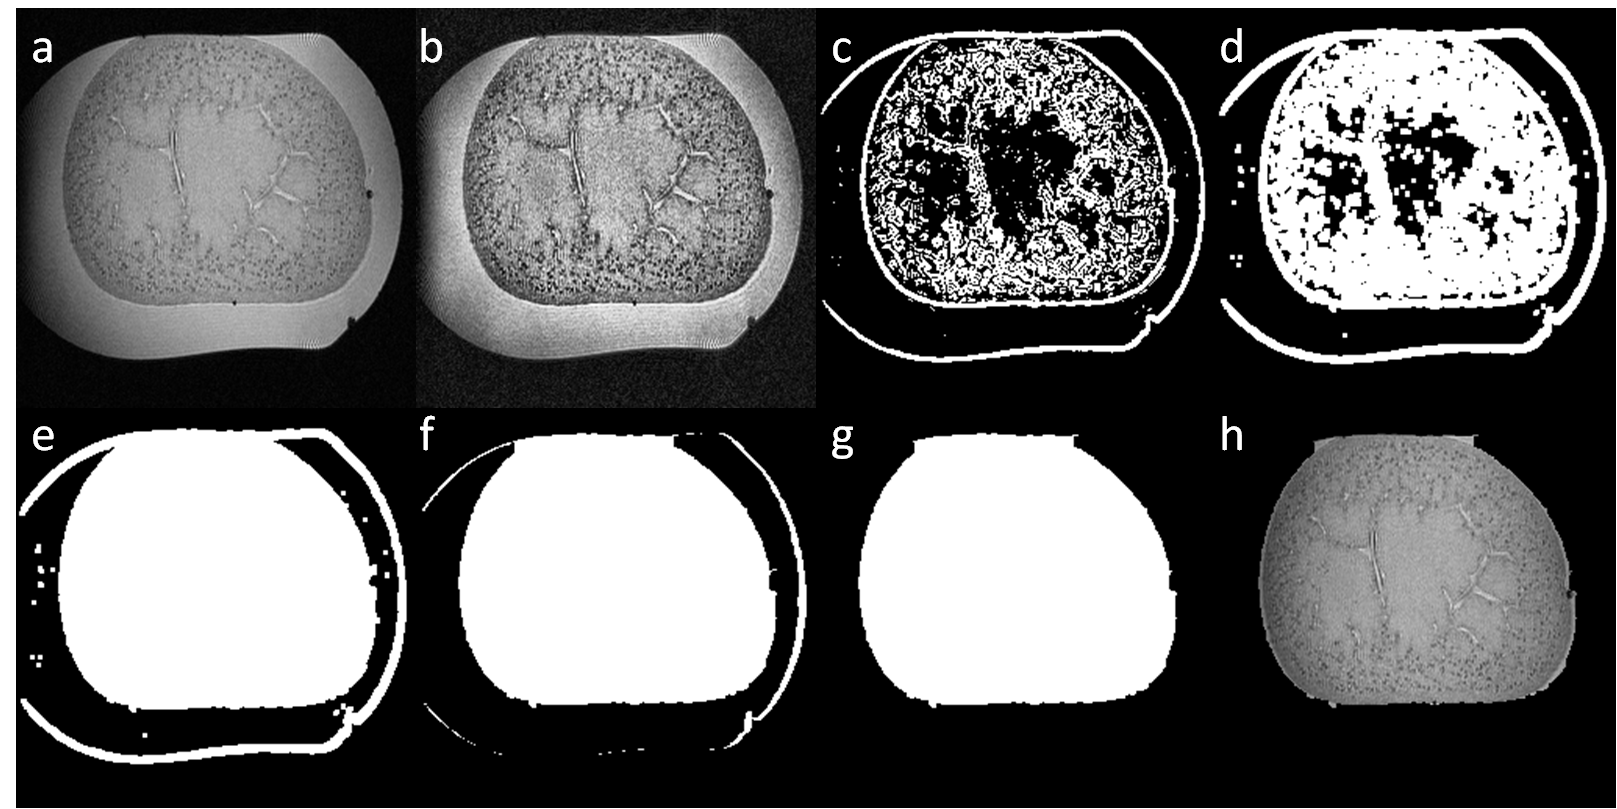
\includegraphics[width=15cm]{group_pic.png}
%\end{minipage}
%\caption{Steps to extract kidney anatomy from the slices. a) Original image, b) image after histogram equalization and subtraction of the background illumination estimate, c) output of Sobel filtering, d) binary image obtained using dilation, e) binary image with filled holes, f) binary image after erosion operation, g) estimated mask obtained using region growing operations, h) extracted kidney. }
%\label{Fig:preprocessing}
%\end{figure*}
%In this section, we describe the proposed algorithm for counting the number of glomeruli in kidney MRI images. In the proposed method, sparse coding based $\ell_1$ graphs are constructed, for patches obtained from the training images, and  projection directions for a low-dimensional embedding are obtained. Note that, a patch is referred as a glomerular patch if its center pixel belongs to a glomerluar region. By incorporating the label information of the patches while learning the embedding, improved discrimination between glomerular and non-glomerular regions can be achieved. The procedure for obtaining the glomerular count involves the following steps: (a) cluster the embedded patches into two classes, (b) create a binary image by assigning the value $1$ to the center pixel of each glomerular patch, and (c) count the number of distinct regions in the binary image.
%
%
%A kidney dataset can have more than two hundred slices to cover the whole kidney anatomy. One of the challenges working with kidney data sets is the intensity non-uniformities across images. The intensity non-uniformities can change the local characteristics of regions within the image, which could in turn make it difficult to correctly identify the regions that contain glomeruli. Hence, we propose to extract the kidney anatomy from the axial slices prior to estimating the glomerular number. We apply well-known morphological operations and filtering methods to mitigate the non-uniformity defects, and create masks that attempt to extract only the kidney anatomy from slices. 
%
%An estimate of the background is generated using a minimum filter on sub-blocks of the image. The output is a low resolution estimate of the background in the image, and the low resolution estimate is upscaled to the original size by bilinear interpolation. Alternatively, a background estimate can be obtained by using morphological opening with a relatively large structuring element. Applying a Sobel filter \cite{DIP1} can provide a binary image which is suitable for employing morphological techniques. In the binary image, the dilation operation fills in most of the area inside the kidney. The rest of the holes are filled using an algorithm based on morphological reconstruction \cite{DIP2}. Following this, erosion and region growing operations are carried out to estimate the final mask. This mask can then be to extract the kidney anatomy from the slice. The steps involved in this process are ilustrated in Figure \ref{Fig:preprocessing}. 
%
%
%\label{sec:l1graph}
%Since constructing an $\ell_1$ graph involves sparse coding, we will review it briefly. In sparse coding, the data is represented as a linear combination of a small set of representative atoms from a dictionary matrix. The dictionary is typically overcomplete, i.e., the number of basis functions exceeds the data dimension and hence we need to solve an underdetermined system of linear equations. The generative model for sparse coding of a data sample $\mathbf{x} \in \mathbb{R}^M$ is given by,
%\begin{equation}
%\label{eqn:gen_model}
%\mathbf{x} = \mathbf{\Psi}\mathbf{a}
%\end{equation} where $\mathbf{\Psi} \in \mathbb{R}^{M \times K}$ is the set of $K$ elementary features and $\mathbf{a} \in \mathbb{R}^K$ is the coefficient vector, which is assumed to be sparse \textit{a priori}. If the data follows the above generative model for some dictionary $\mathbf{\Psi}$, usually sparse regularization results in a more robust recovery compared to other conventional regularization schemes, in inverse problems. It has been shown that sparsity is a reasonable prior for various types of natural signals and images, and hence sparse models are very useful in practice. Sparse codes for data can be obtained using the generative model, either by minimizing the exact $\ell_0$ penalty,
%\begin{eqnarray}
%\hat{\mathbf{a}} = \argmin_\mathbf{a} \|\mathbf{a}\|_0 \text{ subj. to } \mathbf{x} = \boldsymbol{\Psi}\mathbf{a},
%\label{eqn:sc_l0}
%\end{eqnarray} or its convex surrogate $\ell_1$ penalty,
%\begin{eqnarray}
%\hat{\mathbf{a}} = \argmin_\mathbf{a} \|\mathbf{a}\|_1 \text{ subj. to } \mathbf{x} = \boldsymbol{\Psi}\mathbf{a},
%\label{eqn:sc_l1}
%\end{eqnarray}
%where $\|.\|_0$ is the $\ell_0$ norm and $\|.\|_1$ is the $\ell_1$ norm. Since the $\ell_0$ minimization given in (\ref{eqn:sc_l0}) is a combinatorial problem, it is usually replaced by its convex counterpart, the $\ell_1$ minimization.  Since real-world data usually has a noise component and cannot be expressed exactly using the generative model in (\ref{eqn:gen_model}), (\ref{eqn:sc_l0}) and (\ref{eqn:sc_l1}) are posed as penalized estimation problems to take this into account. For instance, (\ref{eqn:sc_l1}) is expressed as,
%\begin{eqnarray}
%\hat{\mathbf{a}} = \argmin_\mathbf{a} \|\mathbf{a}\|_1 + \lambda \|\mathbf{x} - \boldsymbol{\Psi}\mathbf{a}\|_2^2,
%\label{eqn:sc_l1_pen}
%\end{eqnarray} where the regularization parameter $\lambda$ trades off the sparsity and representation error terms.
%
%\begin{figure}[t]
%\begin{minipage}[b]{1.0\linewidth}
%  \centering
%  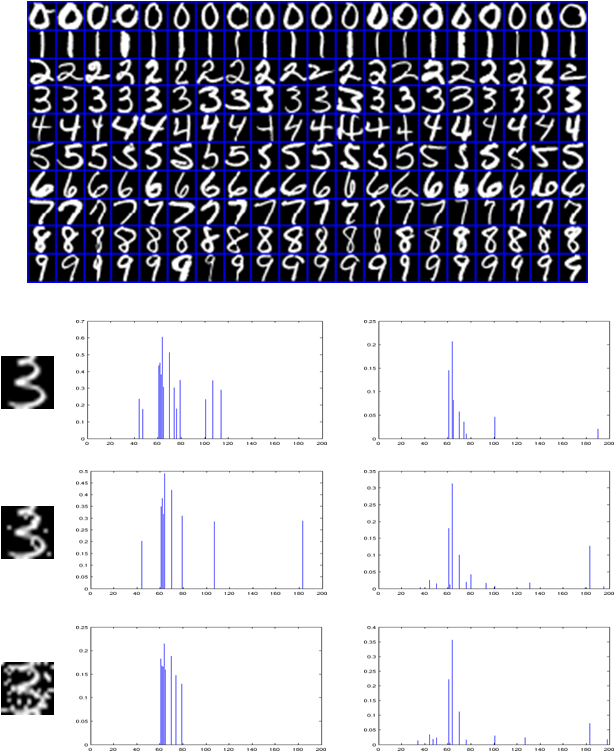
\includegraphics[width=8cm]{l1demo.png}
%\end{minipage}
%\caption{Demonstration of the robustness of an $\ell_1$ graph. The set of training samples used for this simulation are obtained from the USPS dataset \cite{USPSdata}. For an example data sample (Digit $3$), its similarities to all data samples in the case of a K-Nearest Neighbor graph (left) and an $\ell_1$ graph (right) are shown. As the data sample is corrupted by noise, the K-NN graph changes significantly while the $\ell_1$ is robust to the noise.}
%\label{Fig:l1demo}
%\end{figure}
%
%When a set of unlabeled training samples $\mathbf{X} = \{\mathbf{x}_i\}_{i=1}^T$, are available, and each sample can be expressed as a linear combination of a few others from the set, their relationship can be modeled using $\ell_1$ graphs \cite{cheng2010}. In order to obtain this graph, for each data sample $\mathbf{x}_i$, we solve,
%\begin{equation}
%\min_{\mathbf{a}_i} \|\mathbf{x}_i - \mathbf{X} \mathbf{a}_i\|_2^2 + \lambda \|\mathbf{a}_i\|_1 \text{ subj. to } a_{ii} = 0, \mathbf{a}_i \geq \mathbf{0}.
%\label{eqn:l1graph}
%\end{equation}Note that the constraint $a_{ii} = 0$ ensures that $\mathbf{x}_i$ does not contribute to its own representation, and the  non-negativity constraint ensures that the graph weights are non-negative. The $T \times T$ coefficient matrix is constructed as $\mathbf{A} = [\mathbf{a}_1 \mathbf{a}_2 \ldots \mathbf{a}_T]$. We denote the computation of the sparse coefficient matrix using (\ref{eqn:l1graph}) as $\mathbf{A} = \text{SC}(\mathbf{X},\mathbf{X})$, where the arguments denote the data and the dictionary matrices respectively. The Laplacian for the $\ell_1$ graph can be obtained from the coefficient matrix as \cite{wang2009multi}
%\begin{equation}
%\mathbf{L} = (\mathbf{I} - \mathbf{A})^T(\mathbf{I} - \mathbf{A}).
%\label{eqn:lap_l1_graph}
%\end{equation} \textbf{A short derivation of above can be provided, taken from \cite{wang2009multi}.} Here, $\mathbf{I}$ denotes the identity matrix of size $T \times T$. This Laplacian matrix can be subsequently used to perform spectral clustering. In order to demonstrate the robustness of sparse representations, we consider a subset of images from the USPS handwritten digit dataset \cite{USPSdata}. Figure \ref{Fig:l1demo} shows a sample set of images from the USPS dataset. For a given digit image, with varying amounts of noise, similarities are computed using nearest neighbors (left) and sparse coding (right). Clearly, the variation of nearest neighbor similarities is more when compared to sparse coding similarities as the additive noise component increases. Hence the sparse coding graph is more robust to noise when compared to a nearest neighbor graph. \textbf{Intuitively, the Gaussian noise distribution is isotropic, and hence it will affect the local graphs constructed using the isotropic Euclidean distance measure. Whereas, the noise has a very small component along low-dimensional subspaces, and hence they will not affect the relationships in $\ell_1$ significantly.}
%
%The problem of identifying glomeruli in kidney images can be solved using unsupervised clustering with $\ell_1$ graphs. However, such an approach poses two main challenges: (i) prior knowledge about the glomeruli regions cannot be incorporated, and (ii) for each image, $\ell_1$ graphs need to be computed and spectral clustering should be performed, incurring high computational complexity. Hence, we propose to include the label or supervisory information in $\ell_1$ graphs to obtain discriminative, low-dimensional projection directions from a set of training images. For test images, a low-complexity method for estimating the glomerular number is proposed.
%
%In order incorporate supervisory information, we first build a training set by asking an expert to mark the glomerular regions in a few kidney MRI images. The training stage of the algorithm works with image patches of size $5 \times 5$ extracted from the training images. Patches are extracted around every pixel in the image, and those patches centered at the pixels marked as belonging to glomeruli regions are considered to be positive examples ($\mathbf{X}^{+}$). The rest of the patches are the negative examples ($\mathbf{X}^{-}$). This can also be considered as a two class problem, where the positive examples belong to one class and the negative examples belong to another class. The number of positive and negative examples are denoted as $T_p$ and $T_n$ respectively. Our goal is to create a low-dimensional embedding that discriminates the positive and negative examples effectively. We develop an algorithm that uses $\ell_1$ graphs to create supervised embeddings that are robust to noise and intensity variations across images. The training examples are preprocessed by and normalizing them to unit $\ell_2$ norm.
%
%Since we need a discriminative embedding, two $\ell_1$ graphs need to be computed. In the intra-class $\ell_1$ graph, examples belonging to a class are represented by those belonging to the same class. In the inter-class graph, examples belonging to a class are represented by those belonging to a different class. Hence, in order to compute the intra-class graph, we obtain $\mathbf{A}^{(+,+)} =  \text{SC}(\mathbf{X}^{+},\mathbf{X}^{+})$ and $\mathbf{A}^{(-,-)} =  \text{SC}(\mathbf{X}^{-},\mathbf{X}^{-})$. The intra-class coefficient matrix is
%\begin{equation}
%\mathbf{A} = 
%\begin{bmatrix}
%\mathbf{A}^{(+,+)} & \mathbf{0}_{T_p,T_n} \\
%\mathbf{0}_{T_n,T_p} & \mathbf{A}^{(-,-)}
%\end{bmatrix},
%\label{eqn:propwc}
%\end{equation} where $\mathbf{0}$ is a zero matrix with dimensions indicated in the subscript.
%
%To compute the inter-class graph, we need to obtain two coefficient matrices. The elements of the first coefficient matrix, $\mathbf{A}^{(+,-)} \in \mathbb{R}^{T_n \times T_p}$, where each positive example is represented using the set of negative examples are obtained as
%\begin{equation}
%\min_{\mathbf{a}_i} \|\mathbf{x}_i^{+} - \mathbf{X}^{-} \mathbf{a}_i\|_2^2 + \lambda \|\mathbf{a}_i\|_1 \text{ subj. to } \mathbf{a}_i \geq \mathbf{0}.
%\label{eqn:l1graph_inter}
%\end{equation} Repeating this for all $T_p$ positive examples, the shorthand notation for computing the coefficient matrix is $\mathbf{A}^{(+,-)} = SC(\mathbf{X}^{+},\mathbf{X}^{-})$. Similarly the second coefficient matrix for the inter-class graph can be obtained as $\mathbf{A}^{(-,+)} = SC(\mathbf{X}^{-},\mathbf{X}^{+})$. Note that the same shorthand notation when used with the same first and second argument implies computation of intra-class sparse codes using (\ref{eqn:l1graph}). The overall inter-class coefficient matrix is now given by
%\begin{equation}
%\mathbf{A}' = 
%\begin{bmatrix}
%\mathbf{0}_{T_p,T_p} & \mathbf{A}_{(-,+)}  \\
%\mathbf{A}_{(+,-)} &  \mathbf{0}_{T_n,T_n}
%\end{bmatrix}.
%\label{eqn:propbc}
%\end{equation} The intra- and inter-class Laplacian matrices are obtained as
%\begin{align}
%\mathbf{L} &= (\mathbf{I} - \mathbf{A})^T (\mathbf{I} - \mathbf{A}), \\
%\mathbf{L}' &= (\mathbf{I} - \mathbf{A}')^T (\mathbf{I} - \mathbf{A}').
%\end{align}
%
%\begin{figure*}[t]
%\begin{minipage}[b]{1.0\linewidth}
%  \centering
%  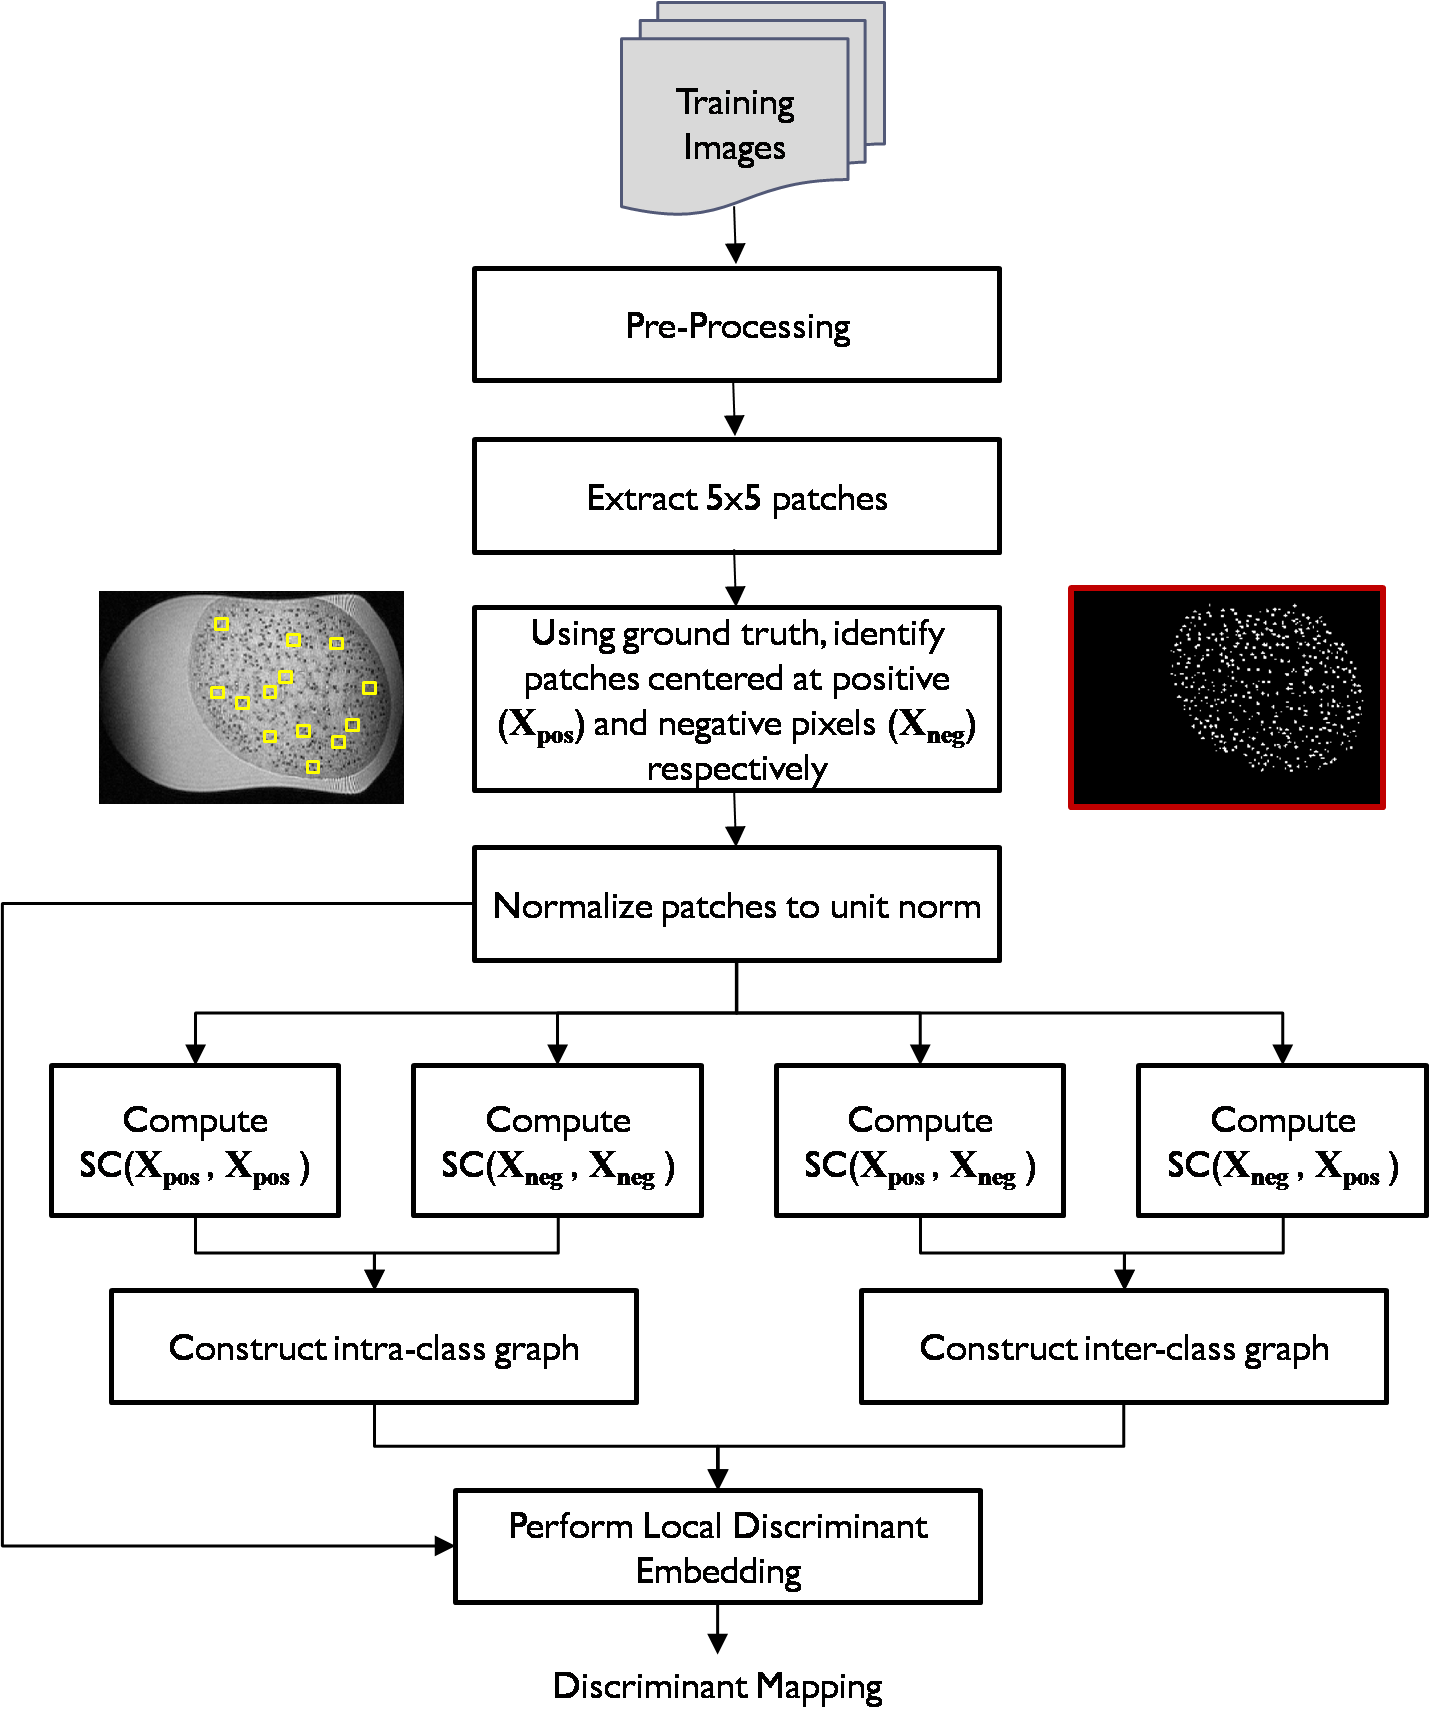
\includegraphics[width=10cm]{train.png}
%\end{minipage}
%\caption{Proposed algorithm for computing an embedding that discriminates image patches containing glomeruli from the rest. This method works by constructing $\ell_1$ graphs to model inter-class and intra-class relationships, and performing local discriminant embedding.}
%\label{Fig:train}
%\end{figure*}
%
%
%Using the intra- and inter-class Laplacians, $\mathbf{L}$ and $\mathbf{L}'$, discriminant embedding directions $\mathbf{V}$ are computed by solving the trace-ratio maximization in (\ref{eqn:ldaopt}). Similar to the case of LDA and LDE, the trace-ratio maximization is simplified as ratio-trace maximization in (\ref{eqn:ldaopt}), which is solved as the generalized eigen decomposition in (\ref{eqn:geneig}). Using the projection directions, the embedding for any training sample $\mathbf{x}$ or test sample, $\mathbf{z}$ can be obtained as $\mathbf{V}^T\mathbf{x}$ or $\mathbf{V}^T\mathbf{z}$ respectively. Figure \ref{Fig:train} describes the process of computing a discriminant embedding using $\ell_1$ graphs. 
% 
%\begin{figure}[t]
%\begin{minipage}[b]{0.99\linewidth}
%  \centering
%  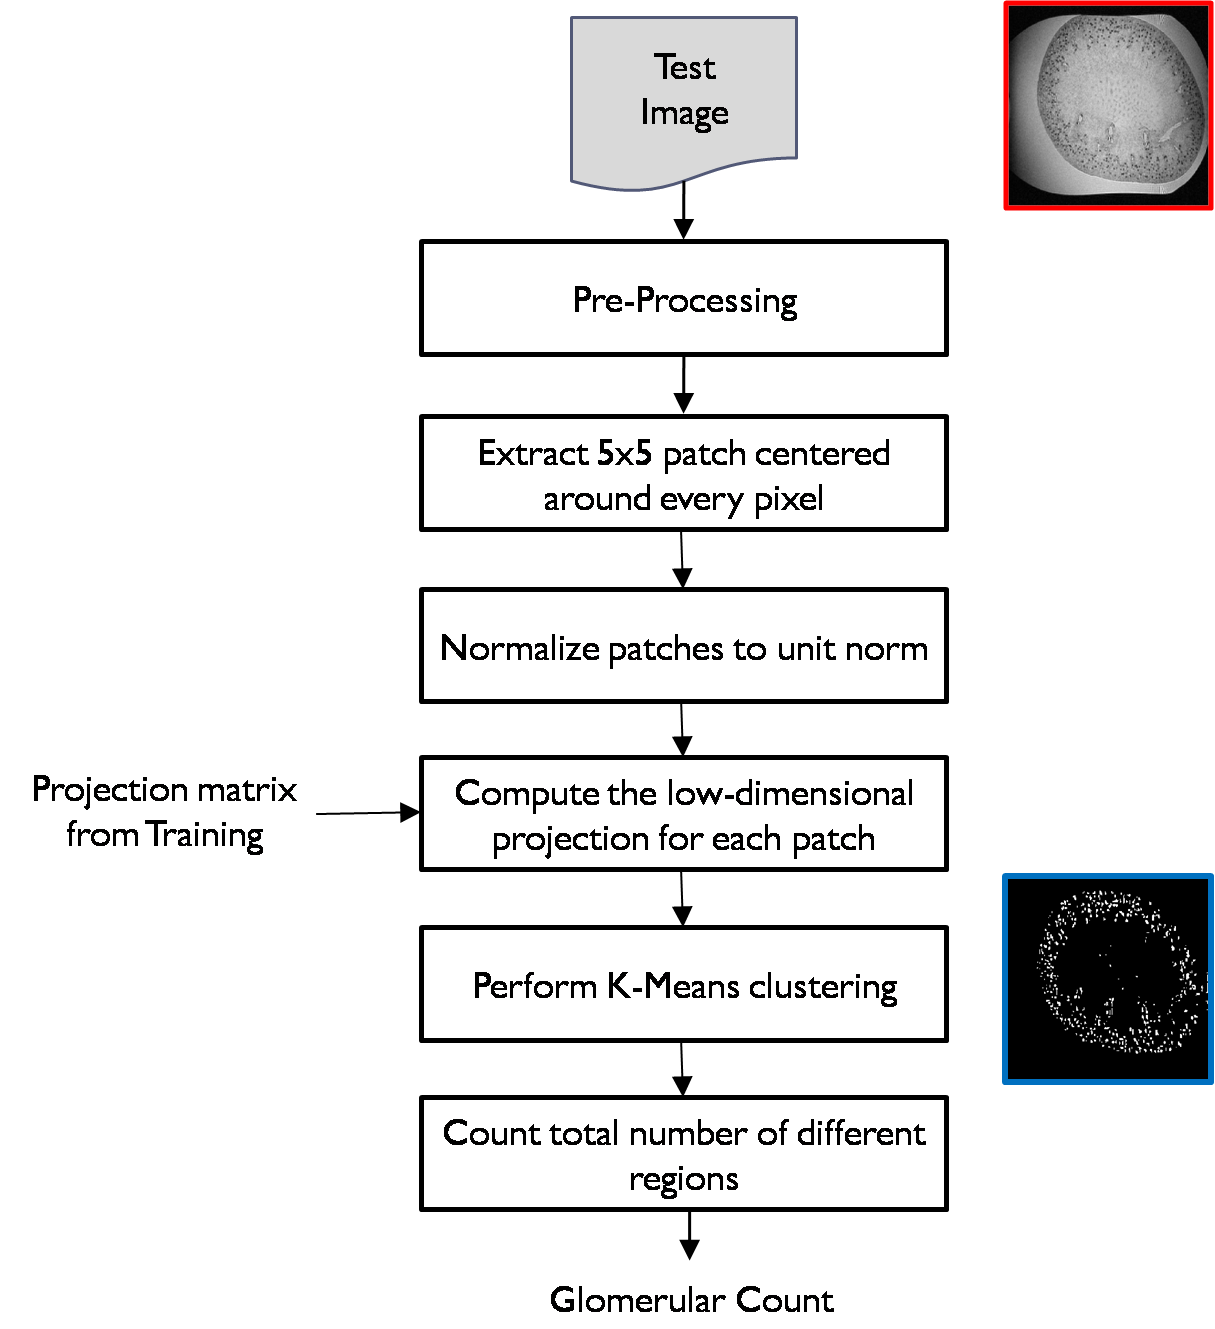
\includegraphics[width=8cm]{test.png}
%\end{minipage}
%\caption{A low-complexity procedure for obtaining the glomerular count in a test image. The discriminant mapping determined in the training stage is used with the test image patches directly, and hence there is no need to obtain the sparse codes for test data.}
%\label{Fig:test}
%\end{figure}
%
%\label{sec:count}
%For a given test images, $5 \times 5$ patches are extracted, their dc component is removed and they are normalized to unit $\ell_2$ norm. The low-dimensional embeddings for these preprocessed set of test patches $\mathbf{Z}$ is obtained as $\mathbf{V}^T \mathbf{Z}$. We employ the K-means procedure to cluster these low-dimensional projections into two groups. The group having smaller number of elements is the one that contains the glomerular regions, since the number of glomerular patches is much smaller compared to the rest. Each patch corresponding to the glomerular cluster is marked in the original test image, and this results in a segmented image. Given this image, we count the number of connected components with at least more than $r$ pixels. This is because we assume that the glomerular regions contain at least $r$ pixels in its neighborhood, so that we can ignore a few lonely false positives provided by the algorithm. Since the proposed algorithm uses only simple matrix multiplication and clustering in low-dimensions, it is computationally efficient. The steps involved in obtaining the glomerular count for a test image are illustrated in Figure \ref{Fig:test}.